%------------------------------------------------------------------------%
\chapter{Diodes}
%------------------------------------------------------------------------%
Diodes or pn junction are basically 2 zones of opposite doping polarity attached toghether.\\
To study pn junctions we have to make some simplyfing assumptions : we consider 1D materials with constant doping concentration and a step-like change of doping.\\
%------------------------------------------------------------------------%
\section{Built-in potential}
%------------------------------------------------------------------------%
\begin{wrapfigure}{i}{0pt}
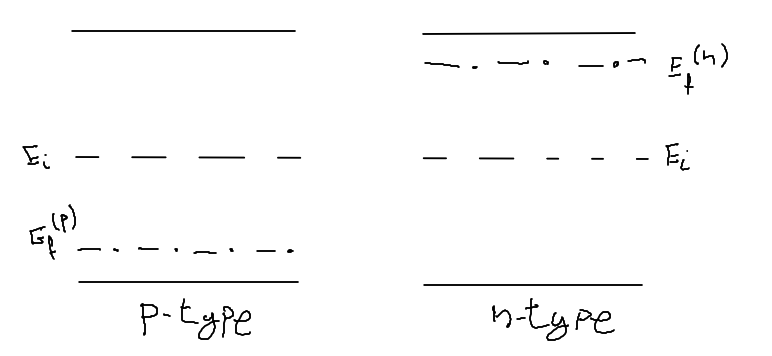
\includegraphics[width=0.4\textwidth]{pn1.png}
\end{wrapfigure}


Let's consider the 2 regions isolated from each other and under th.eq. We don't have a single Fermi level so depending on the zone we have 
\begin{equation}
E_i-E_f^{(n)}=kT\ln(\frac{N_a}{n_i}) \ \ \ \ \ \ \ E_f^{(n)}-E_i=kT\ln(\frac{N_d}{n_i})
\end{equation}
where $E_f^{(n/p)}$ is the Fermi level in that zone.\\

\begin{wrapfigure}{o}{0pt}
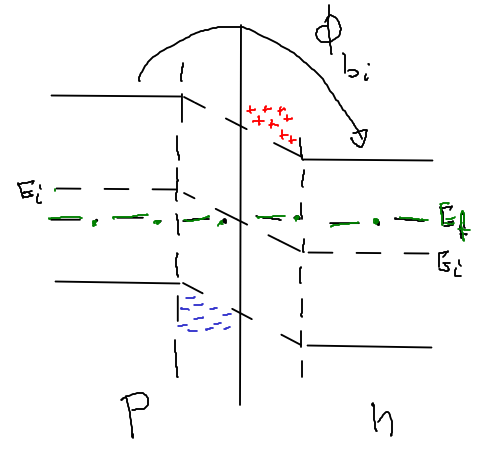
\includegraphics[width=0.25\textwidth]{pn2.png}
\end{wrapfigure}

When we put the 2 materials toghether there will be first a diffusion current and than olso a drift current due to the band banding and the exposed charge; we will reach th.eq when the total current will be 0.\\Under th.eq we will have a costant Fermi level all over the space and a band banding at the interface. Far from the intarface we will reach zones where the bands are like the isolated case. The drop of electrostatic potential in the junction under th.eq is called built in potential or $\phi_{bi}$ and is 
\begin{equation}
q\phi_{bi}=(E_f^{(n)}-E_f^{(p)})|_{n.e}=kT\ln(\frac{N_aN_d}{n_i^2})
\end{equation} 
that is close to the $E_g$ of the material.\\
%------------------------------------------------------------------------%
\section{Depletion approximation}
%------------------------------------------------------------------------%
Beacuse the distance $E_f-E_c$ increase near the junction we have a exponential deacrease of n so in the transition region we can say that $n<<N_d$ and so $p<<N_a$.\\
From this we can say that the transition region is depleted of free carriers beacuse their concentration is negligible so this region is called depletion region.
%------------------------------------------------------------------------%
\section{Electrostatics of a pn junction}
%------------------------------------------------------------------------%

\begin{wrapfigure}{i}{0pt}
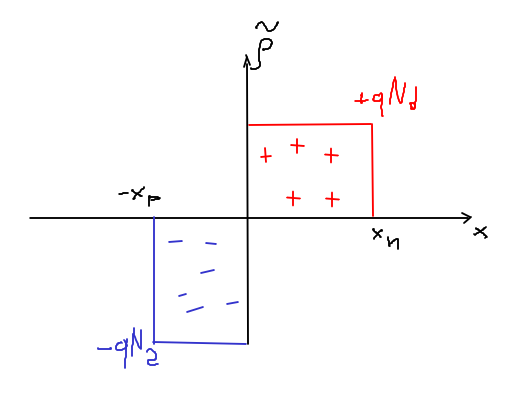
\includegraphics[width=0.35\textwidth]{pn3.png}
\end{wrapfigure}

We have to solve poisson equation in the depletion region so using depletion approximation and considering complete ionization
\begin{equation}
\frac{d\phi^2}{dx^2}=-\frac{q}{\varepsilon}(N_d-N_a)
\end{equation} 
and considering the concentration of fixed charges like the graph we can split the Poisson eq in 2 parts for $-x_p<x<0$ we have $\frac{d\phi^2}{dx^2}=\frac{q}{\varepsilon}N_a$ and for $0<x<x_n$ we have $\frac{d\phi^2}{dx^2}=-\frac{q}{\varepsilon}N_d$.\\
If we integrate both side of this equation and remembering that $F(x_n)=0$ we can deduce the electric field in the junction as 
\begin{equation}
\int^{x_n}_{x} d\frac{d\phi}{dx}=\int^{x_n}_{x}-\frac{q}{\varepsilon}N_d dx
\end{equation}

\centering
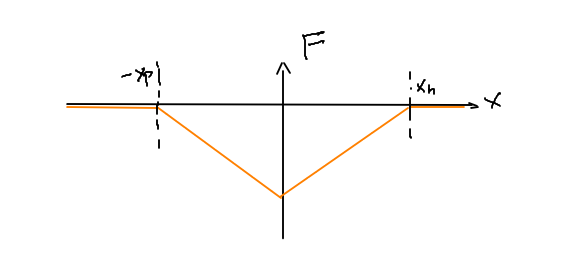
\includegraphics[width=0.35\textwidth]{pn4.png}\\
\raggedright

\begin{equation}
F(-x_p<x<0)=-\frac{qN_a}{\varepsilon}(x_p+x)\ \ \ \ \ \ \ \ F(0<x<x_n)=-\frac{qN_d}{\varepsilon}(x_n-x)
\end{equation}

\begin{wrapfigure}{i}{0pt}
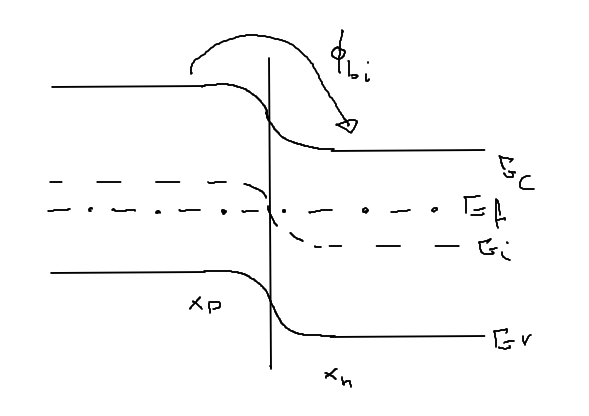
\includegraphics[width=0.3\textwidth]{pn5.png}
\end{wrapfigure}

for continuity equations of the electric field the F must be continuos in 0 so from this condition we get that $N_ax_p=N_dx_n$ that means that the total charge in the depletion area is 0 (from Gauss law olso).\\
Integrating again both parts of the equation of the field we finally obtain the potential over the space that has a parabolic dependance
\begin{equation}
\phi(-x_p<x<0)=\phi(-x_p)+\frac{qN_a}{2\varepsilon}(x+x_p)^2 \ \ \ \ \ \ \ \ \phi(0<x<x_n)=\phi(x_n)-\frac{qN_d}{2\varepsilon}(x_n-x)^2
\end{equation}


To know $x_n$ and $x_p$ we have to set some boundary condition: $\phi$ must be continuos in 0, and $N_ax_p=N_dx_n$ from this 2 condition we get 
\begin{equation}
x_n=\sqrt{\frac{2\varepsilon}{q}\phi_{bi}(\frac{1}{N_a}+\frac{1}{N_d})}\times \frac{N_a}{N_a+N_d}\ \ \ \ \ \ \ 
x_p=\sqrt{\frac{2\varepsilon}{q}\phi_{bi}(\frac{1}{N_a}+\frac{1}{N_d})}\times \frac{N_d}{N_a+N_d}\ \ \ \ \ \ \ 
W=\sqrt{\frac{2\varepsilon}{q}\phi_{bi}(\frac{1}{N_a}+\frac{1}{N_d})}
\end{equation}

%------------------------------------------------------------------------%
\section{Unilateral Junction}
%------------------------------------------------------------------------%

\begin{wrapfigure}{i}{0pt}
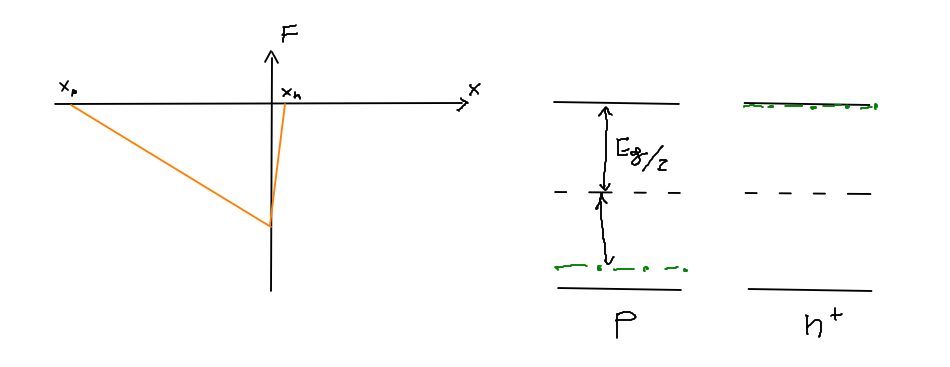
\includegraphics[width=0.6\textwidth]{pn6.png}
\end{wrapfigure}

Let's consider a junction $n^+p$ so the depletion area is almost all in the less doped material and so the electric field. We can make some approximation that the depletion area is almost in the p zone and that the Fermi level of the $n^+$ zone is almost at $E_c$ so this lead us to 
\begin{equation}
W\simeq x_p \ \ \ \ \ q\phi_{bi}\simeq E_g/2 + kT\ln(\frac{N_a}{n_i})
\end{equation}

%------------------------------------------------------------------------%
\section{Bias}
%------------------------------------------------------------------------%
{\bf Forward Bias}\\

\centering
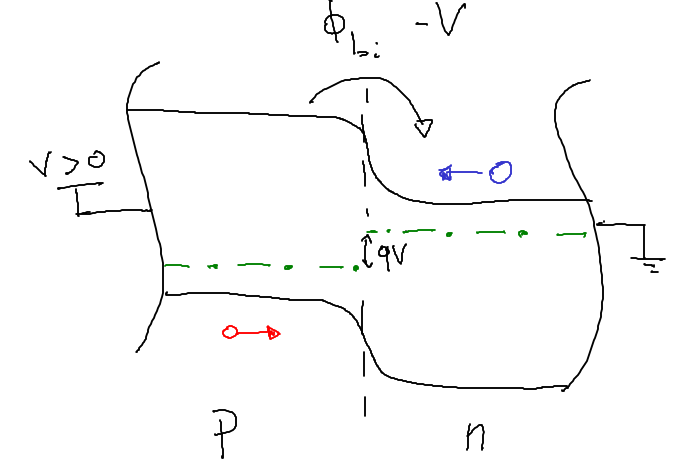
\includegraphics[width=0.35\textwidth]{pn7.png}\\
\raggedright

Applying a external voltage like in figure we are reducing the total voltage drop over the junction. There will be a net flow of electrons from left to right that is a current by diffusion that will be large beacuse we have a lot of charges.\\
{\bf Revers Bias}\\

\centering
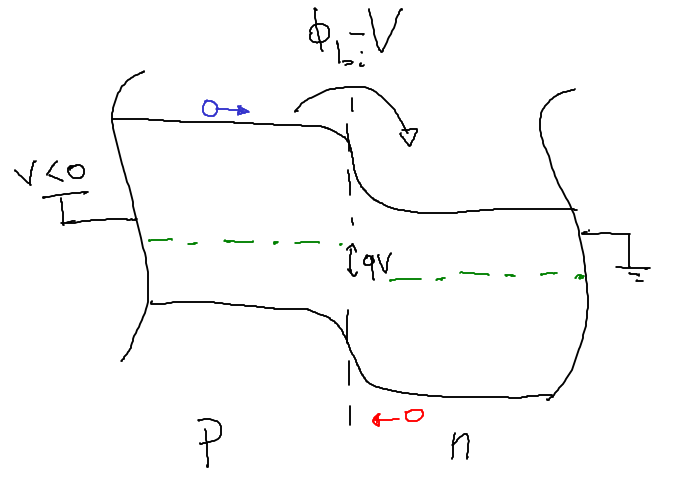
\includegraphics[width=0.35\textwidth]{pn8.png}\\
\raggedright

In this case $V<0$ electrons and holes move for drift the total voltae drop is will be greater than the built in. The flow of current is given by minority carrier so small I.\\

%------------------------------------------------------------------------%
\section{The V-I characteristic of pn }
%------------------------------------------------------------------------%
First we want to investigate on foward bias electrostatic but we have to make some other simplyfing assumption: the contacts of our junction are at th.eq. and looking to the n region moving closer to the contact (from the interface) we will enter in a region where electrons are majority carrier. Beacuse we are injecting holes in that region we will have $p=p_{n0}+\Delta p$ so a region of quasi-equilibrium.\\
If we assume stationarity and that G and R process are negligible and so the $J_n=n\mu_n \frac{dE_{fn}}{dx}=cost$ so beacuse n isn't costant all over the space (space of all the diod first n minority than majority) $\frac{dE_{fn}}{dx}$ will change over the space.
The final graph is this 

\centering
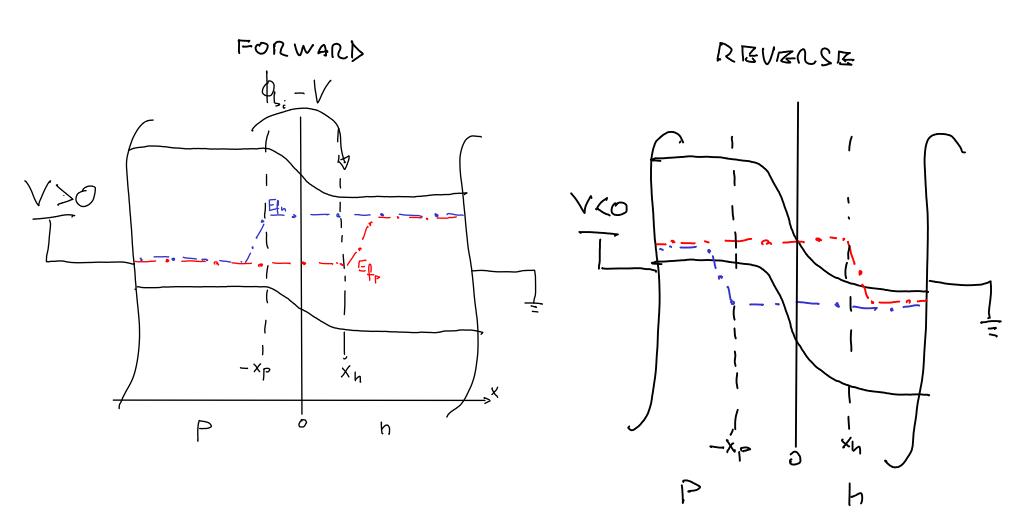
\includegraphics[width=0.6\textwidth]{pn9.png}\\
\raggedright

we have 2 region of quasi-equilibrium and a transition region that is depleted from free charges. This is the same result of electrostatic without bias so the depletion region will be
\begin{equation}
W=\sqrt{\frac{2\varepsilon}{q}(\phi_{bi}-V)(\frac{1}{N_a}+\frac{1}{N_d})}
\end{equation}
$E_{fn}$ remains costant until $-x_p$ but n changes beacuse $E_c$ moves upwards.\\
For reverse bias we have to follow the same path of forward bias arriving at the graph above.\\
Bands are flat near the contact beacuse we suppose (1) quasi-neutral region under (2) low level of injection with (3) costant doping and (4) negligible gradient of quasi-Fermi levels; if one of this supposition falls the bands will no more be flat.\\
\vspace{5mm}
\label{cont.eq}
Now we want to know the quasi-Fermi level in the minority region.
We know that at $x=x_n$ $n\simeq N_d$ and for the law of mass action generalized $p=\frac{n_i^2}{n}e^{\frac{E_{fn}-E_{fp}}{kT}}\simeq p_{n0}e^{\frac{qV}{kT}}$ and at $x=-x_p$ with the same passages we obtain $n\simeq n_{p0}e^{\frac{qV}{kT}}$. Now we can solve the continuity equation only in the quasi-neutral region. \\
Beacuse the bands are flat we have only diffusion so $J_n=qD_n \frac{dn}{dx}$ and $G-R=\frac{-\Delta n}{\tau_n}$ from this two in the coninuity equations under stationary condition we get
\begin{equation}
\frac{d^2\Delta n}{dx^2}-\frac{\Delta n}{L_n^2}=0
\end{equation} 
where $L_n=\sqrt{D_n\tau_n}=$ diffusion length of electrons in the quasi neutral p-region. Introducing the system of coordinate like in figure (where $W_p$ is the end of the quasi-neutral p region) we can solve this differential equation.

\begin{wrapfigure}{i}{0pt}
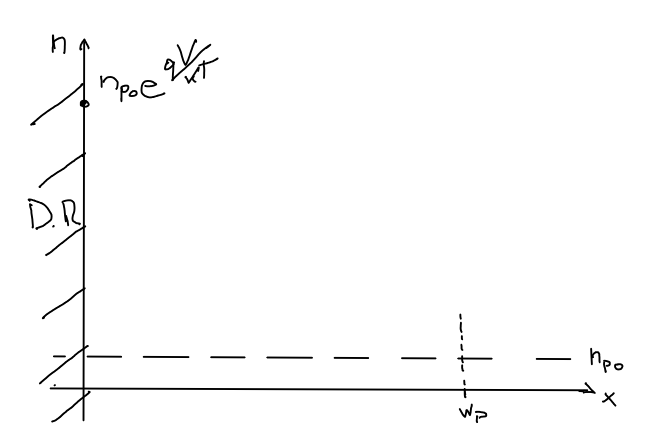
\includegraphics[width=0.45\textwidth]{pn10.png}
\end{wrapfigure}

Solving that as a polynomial we get $\lambda^2-\frac{1}{L_n^2}=0\leftarrow \lambda=\pm\frac{1}{L_n}$ so we get two exponential terms that are $\Delta n(x)=Ae^{\frac{x}{L_n}}+Be^{-\frac{x}{L_n}}$ using the boundary condition $\Delta n(0)=n_{p0}(e^{\frac{qV}{kT}}-1)$ and $\Delta n(W_p)=0$ we arrive at
\begin{equation}
\Delta n(x)=n_{p0}(e^{\frac{qV}{kT}}-1)\frac{\sinh(\frac{W_p-x}{L_n})}{\sinh(\frac{W_p}{L_n})}
\end{equation}
Having only diffusion processes we can know the current but we are intrested only in $J_n(0)$ at the edge of the quasi-neutral region so 
\begin{equation}
J_n(0)=(qD_n \frac{d\Delta n}{dx})|_{x=0}=-\frac{qD_nn_{p0}}{L_n\tanh(W_p/L_n)}(e^{\frac{qV}{kT}}-1)
\end{equation}
so in general the total current in the pn junction is 
\begin{equation}
J=[\frac{qD_nn_{p0}}{L_n\tanh(W_p/L_n)}+\frac{qD_pp_{n0}}{L_p\tanh(W_n/L_p)}](e^{\frac{qV}{kT}}-1)=J_0(e^{\frac{qV}{kT}}-1)
\end{equation}

\begin{wrapfigure}{i}{0pt}
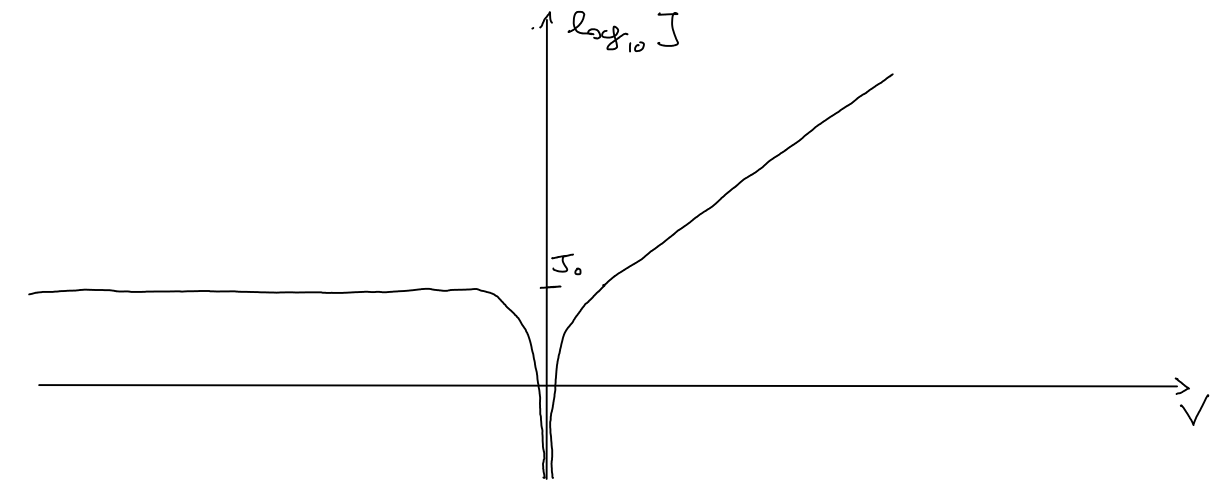
\includegraphics[width=0.35\textwidth]{pn11.png}
\end{wrapfigure}


If $V>>kT/q$ we can neglect 1 and plot a log-log scale of this characteristic that is 
\begin{equation}
\log(J)=log(J_0)+\frac{qV}{kT\ln(10)}
\end{equation}
One important parameter of the characteristic is the slope in foward bias that is $kT/q \ln(10)=60mV/dec \ @RT$.\\
The dominant contribute to the current is from the zone less doped like in the electrostatic.\\

%------------------------------------------------------------------------%
\section{Wide and narrow base diode}
%------------------------------------------------------------------------%

\centering
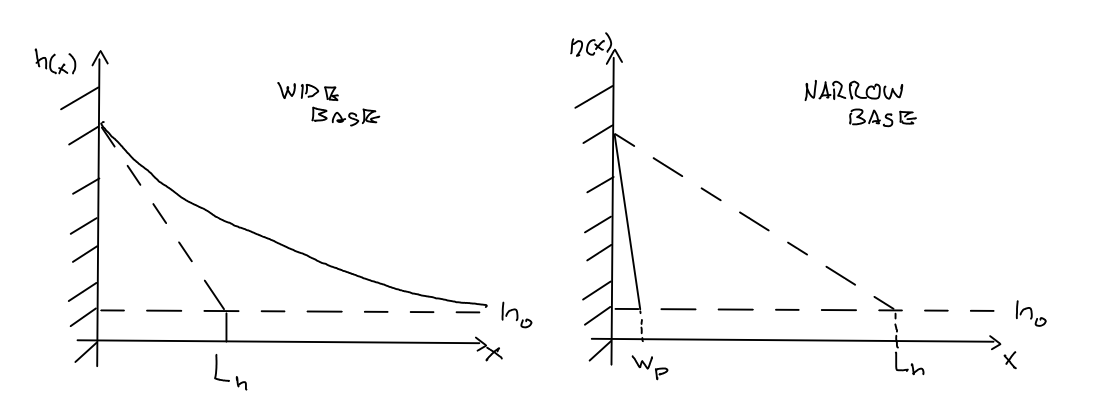
\includegraphics[width=0.65\textwidth]{pn12.png}\\
\raggedright

If we have a wide-base diode if $W_p>>L_n$ so we can approximate as follow the expression of charge and of current density 
\begin{equation}
\Delta n(x)=n_{p0}(e^{\frac{qV}{kT}}-1)e^{\frac{-x}{L_n}} \ \ \ \ \ \ \ J_n=\frac{qD_nn_{p0}(e^{\frac{qV}{kT}}-1)}{L_n}
\end{equation}


If we have a narrow-base diode if $W_p<<L_n$ so we can approximate as follow the expression of charge and of current density
\begin{equation}
\Delta n(x)=n_{p0}(e^{\frac{qV}{kT}}-1)\frac{W_p-x}{W_p}\ \ \ \ \ \ \ \ \ J_n=\frac{qD_nn_{p0}(e^{\frac{qV}{kT}}-1)}{W_p}
\end{equation}


\begin{wrapfigure}{i}{0pt}
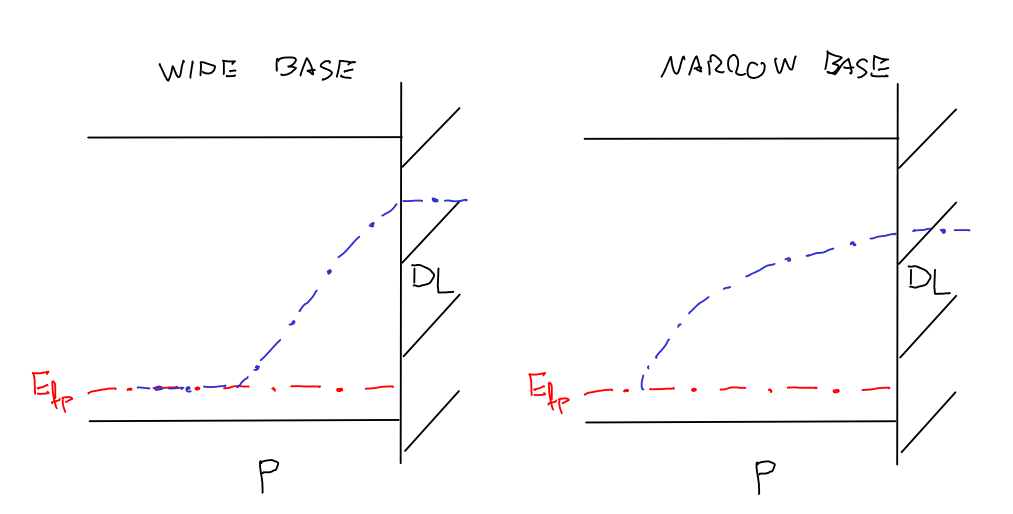
\includegraphics[width=0.35\textwidth]{wbnb.png}
\end{wrapfigure}

In a wide base diode n(x) decrease exponentially in the p region therefore $E_{fn}$ will decrease linearly with a slope of $kT/L_n$ and after the intersection with $E_{fn}$ it will be costant as this last one.\\
For a narrow base the decrease of $E_{fn}$ will be logaritmic beacuse n(x) decreases linearly.\\
In the quasi neutral p (n) region we have less electrons (holes) than in all other zone so the highest resistivity. The limit for conduction is given by the quasi-neutral region where we have less concentration of minority carriers; this is why the pn junction is called a minority carriers device , the limit for current transport is given by minority carriers.\\

\subsection{Current profile}
%------------------------------------------------------------------------%
{\bf Wide base forward bias}\\
The exponential behaviour of the minority will be followed by a consequent increase of majority charges in order to mantain the region quasi-neutral. In the depletion layer a connection between the 2 region. Minority carriers moves for diffusion but majority carrier moves for drift beacuse there is a small gradient of $E_{fn}$ that let electrons move from right to left.

\centering
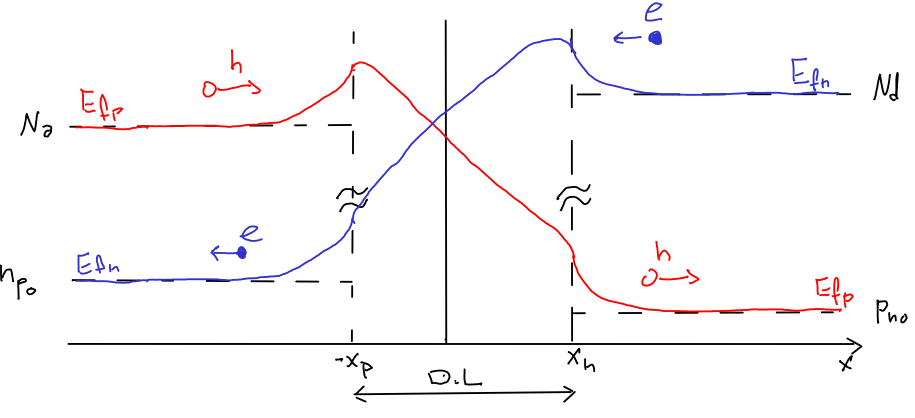
\includegraphics[width=0.5\textwidth]{nxfvb.png}\\
\raggedright

To know $J_n$ in n region we have to remember that under stationary condition (so in quasi neutral region) $J_n+J_p=const$. Olso we remember that under stationary conditions and neglecting G-R both current contributions are constant. From this considerations we can draw the graph of $J_n,J_p$ over the space.\\

\centering
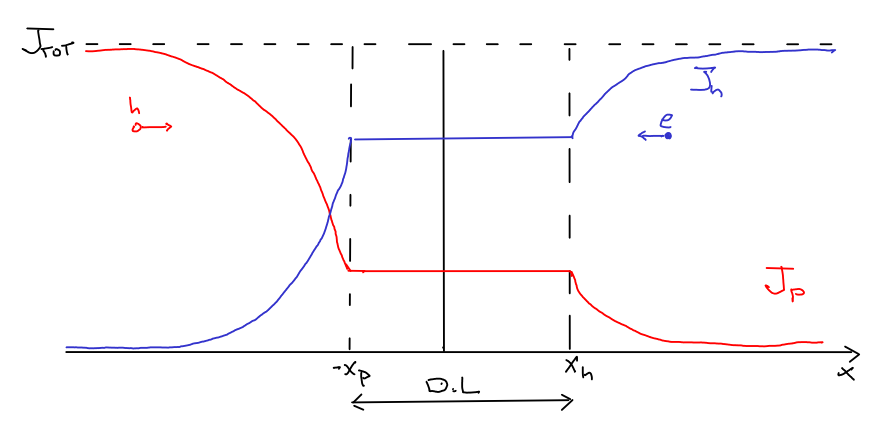
\includegraphics[width=0.5\textwidth]{wbfbJ.png}\\
\raggedright

{\bf Wide base reverse bias}\\
Same path of before : minority carrier in quasi neutral regions decrease before the depletion layer so this phenomena will be copied by the majority carrier in order to mantain quasi-neutrality.

\centering
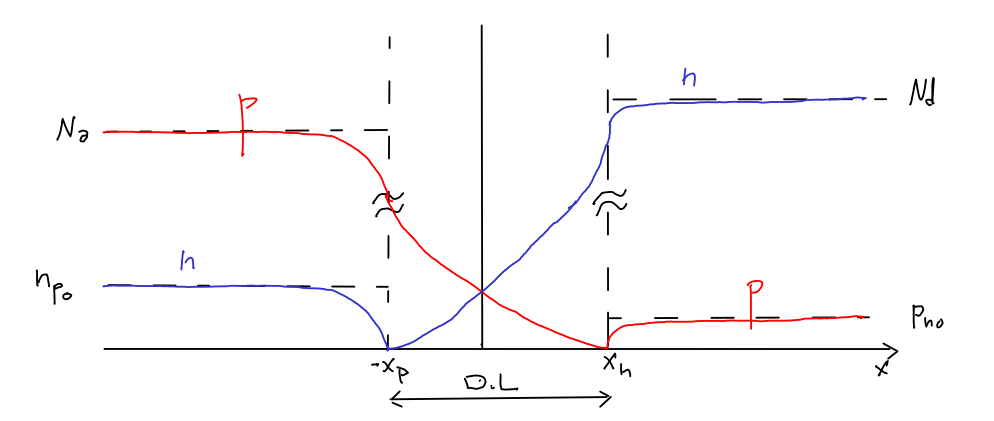
\includegraphics[width=0.5\textwidth]{rbwb.png}\\
\raggedright

Knowing $J_n+J_p=const$ in stationary conditions and that if we neglect olso G-R process we have both currents constat we obtain the following graph.

\centering
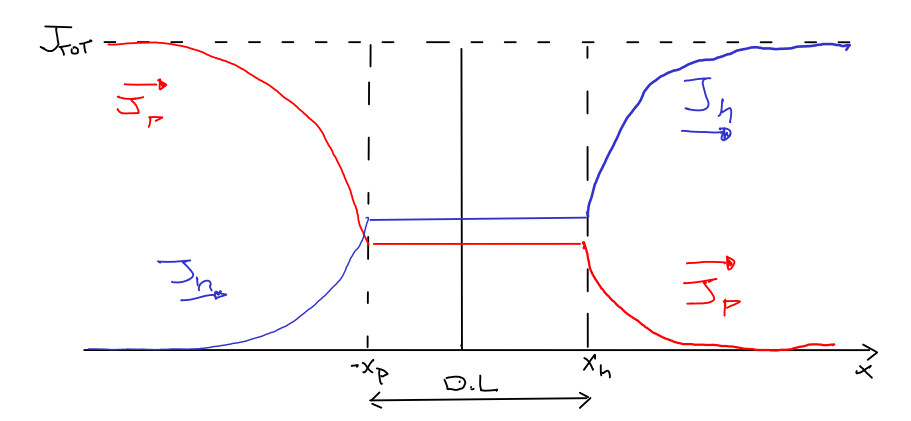
\includegraphics[width=0.5\textwidth]{wbrb.png}\\
\raggedright

The flow of holes becomes zero at n contact but than in grows for generation processes.\\
We have the same behaviour of the current both in reverse and in forward bias but $J_{tot}$ changes of orders of magnitude. As before minority carriers move by diffusion, majority by drift and in the depletion layer we have movement by drift.\\

{\bf Narrow base forward bias}\\
Linear increase of minority carriers so olso majority in order to mantain the region quasi-neutral.\\

\centering
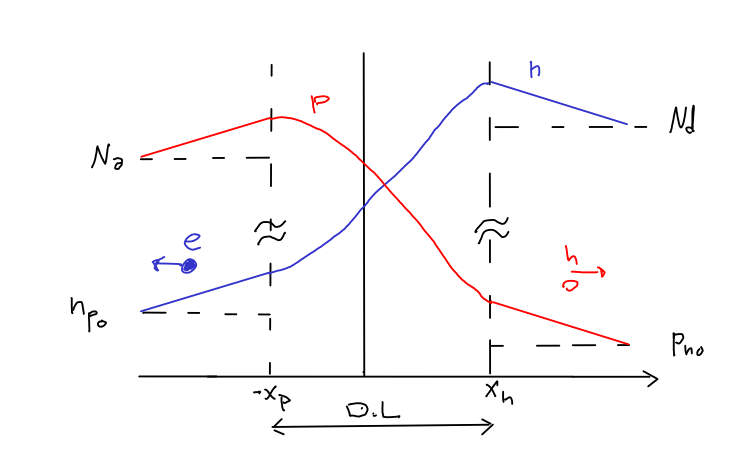
\includegraphics[width=0.5\textwidth]{nbfb.png}\\
\raggedright

The derivate of a linear dependence is constat so $J_n$ and $J_p$ remain constat. There is no space to G-R process beacuse the device is much shorter than $L_n$ so all generation and ricombination process are at the contacts.\\


\centering
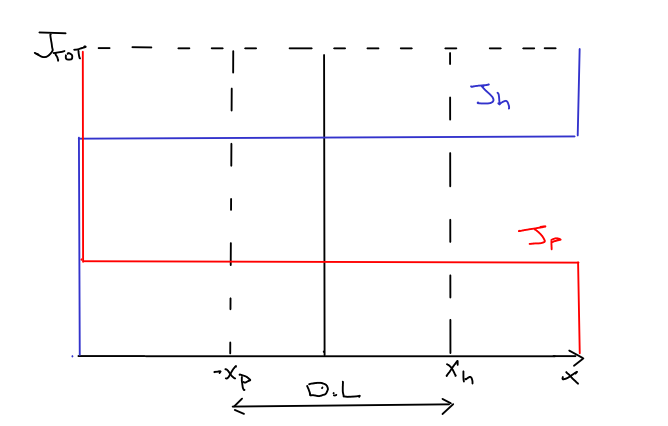
\includegraphics[width=0.5\textwidth]{nbJf.png}\\
\raggedright

{\bf Narrow base reverse bias}\\
With the same path of before we arrive at

\centering
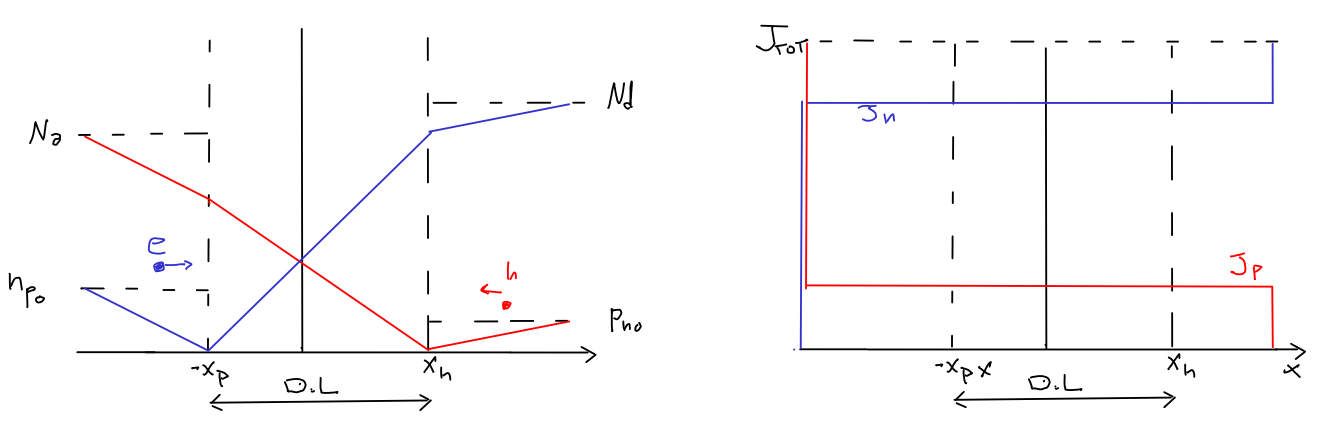
\includegraphics[width=0.85\textwidth]{nwall.png}\\
\raggedright

%------------------------------------------------------------------------%
\section{T change}
%------------------------------------------------------------------------%
Let's consider a pn junction in foward bias $J=J_0(e^{\frac{qV}{kT}}-1)\simeq J_0e^{\frac{qV}{kT}}$. If we increase the T the slope of the straight part will increase for the exponential term (be careful to units in the graph the line becomes flatter) but olso $J_0=\frac{qD_nn_i^2}{N_aL_n}$ will increase for his strong dependance with temperature caused by $n_i^2\propto T^3e^{-\alpha/T}$.

\begin{wrapfigure}{i}{0pt}
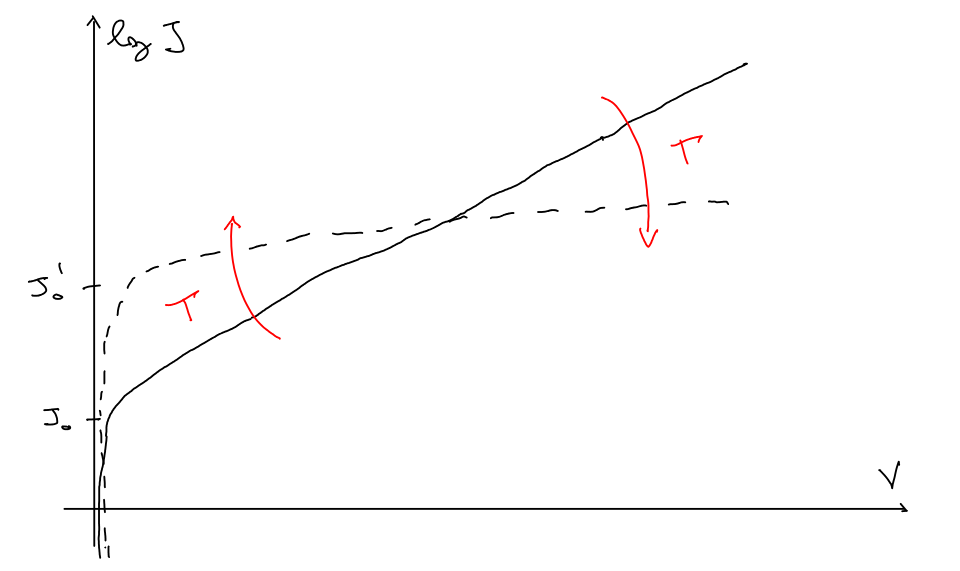
\includegraphics[width=0.5\textwidth]{JwithT.png}
\end{wrapfigure}

So with the increase of T we can have both an increase or a decrease of voltage corrisponding a fixed J. We have to find the typical regime of our device so from $J=J_0e^{\frac{qV}{kT}}$ we extract the voltage as $V=\frac{kT}{q}\ln(J/J_0)$ with J a fixed current. Now we cand derivate obtaining

\begin{equation}
\frac{dV}{dT}= \frac{k}{q}\ln(J/J_0)+\frac{kT}{q}J_0/J \frac{-J \frac{dJ_0}{dT}}{J_0^2}=V/T-\frac{kT}{q}\frac{dJ_0}{dT}\frac{1}{J_0}
\end{equation}

for semplicity we can hilight $J_0$ dependences on temperature writing $J_0=aT^\gamma e^{-E_g/2kT}$ so we obtain that $\frac{dJ_0}{dT}=J_0\gamma/T+J_0[-\frac{dE_g}{dT}\frac{1}{kT}] + J_0 \frac{E_g}{kT^2}$ so coming back at voltage we obtain

\begin{equation}
\frac{dV}{dT}=(V-\frac{E_g}{q})\frac{1}{T}-\frac{k\gamma}{q} + \frac{1}{q}\frac{dE_g}{dT}
\end{equation}

Since our typical $V\simeq0.6/0.7$ there are all negative terms so we are in the firs zone where we find a decrease of voltage w.r.t an increase of the temperature ( at RT $dV/dT\simeq -1.9mV/K$)

%------------------------------------------------------------------------%
\section{Second order effects on current}
%------------------------------------------------------------------------%
There are some phenomena that we have to consider in order to make more realistic the J-V graph of a pn junction.
%------------------------------------------------------------------------%
\subsection{Low current regime}

\begin{wrapfigure}{i}{0pt}
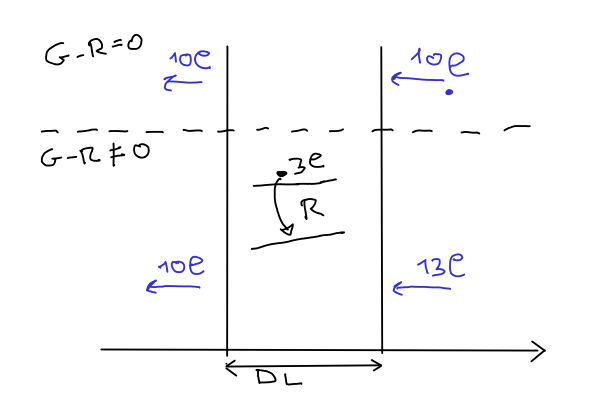
\includegraphics[width=0.35\textwidth]{Rdl.png}
\end{wrapfigure}

We have always neglect the G-R in the depletion layer but now we have to make some considerations.\\
Under reverse bias $E_{fn}<E_{fp}$ so there will be some generation processes, knowing the quasi-Fermi level and using the law of mass action generalized we can write the SRH R coefficient as
\begin{equation}
R=\frac{n_i^2(e^{(qV)/(kT)}-1)}{\tau_0(p+n+2n_i Ch((E_t-E_i)/(kT))}
\end{equation} 
so the sign of the voltage applied V change the sign of R.\\
Refering to forward bias the impact of R is that from majority region there will be more electron moving to the depletion region beacuse of minority constrain of the pn junction. 
So we aspect a larger current under foward bias where $R\simeq \frac{n_i^2(e^{\frac{qV}{kT}}-1)}{\tau_0[p+n]}$ to get the worst case we take p=n so R will be maximum and we get $R= \frac{n_i(e^{\frac{qV}{2kT}})}{2\tau_0}$.\\
Under forward bias so we can define 
\begin{equation}
J_R=qR_{max}W_d=qW_d\frac{n_i(e^{\frac{qV}{2kT}})}{2\tau_0}
\end{equation}
Under reverse bias $R\simeq -\frac{n_i^2}{2n_i\tau_0}=-\frac{n_i}{2\tau_0}$ and so as for forward bias we can define
\begin{equation}
J_G=-q\frac{n_i}{2\tau_0}W_d
\end{equation}
In general for both cases we can define 
\begin{equation}
J_{GR}=\frac{qn_i}{2\tau_0}W_d(e^{\frac{qV}{2kT}}-1)=J_{0GR}(e^{\frac{qV}{2kT}}-1)
\end{equation}

\centering
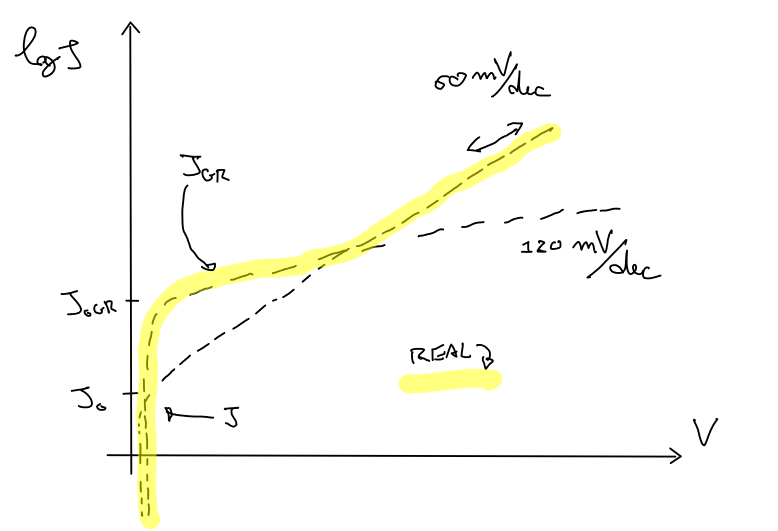
\includegraphics[width=0.5\textwidth]{lowcurrent.png}\\
\raggedright

Similar to ideal but $J_{0GR}$ is bigger and we have a factor 2 at the exp so there is a slight difference at very low current.
Note that $J_{0GR}\propto 1/\tau_0$ so is very process dependent and olso that the ideal $J_0$ has a quadratic dependance on $n_i$ (and this term has a linear dependance) so at high temperature we recover the ideal diode characteristic.\\ 
With reverse bias the current is dominated by $J_{RG}$ and have a slight increase due to the dependence of $W_d$ with V.\\

\centering
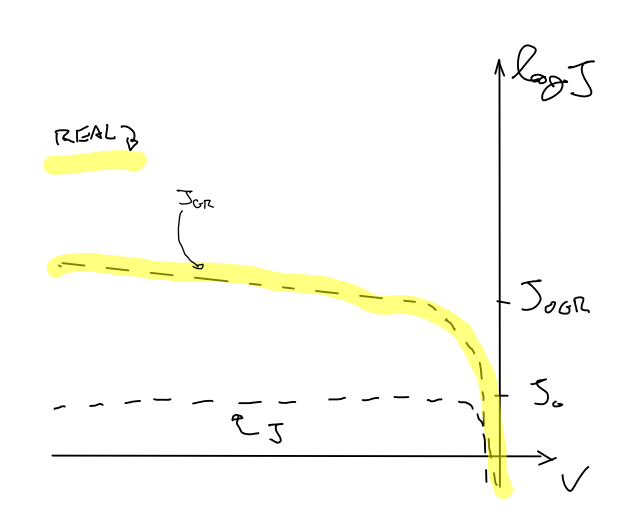
\includegraphics[width=0.35\textwidth]{inverselow.png}\\
\raggedright

\subsection{High current regime}
At high current regime there are 2 problems that create distortion in the ideal characteristic.\\
{\bf High injection regime}\\
At high current the hypotesis of low injection regime decades so taking p quasi-neutral region we have $n=n_0+\Delta n\simeq\Delta n$ and $p=p_0+\Delta n\simeq \Delta n$ so with the law of mass action generalized we obtain $pn=n_i^2e^{\frac{qV}{kT}}=\Delta n^2$ and so $\Delta n=n_ie^{\frac{qV}{2kT}}$ from this through continuity equation (see ~\ref{cont.eq}) we get that 
\begin{equation}
J\propto n_ie^{\frac{qV}{2kT}}
\end{equation}
so an additional solpe of 120mv/dec.\\ 
{\bf Resistive drops}\\
$E_f$ gradient is no more negligible so we have parasitic resistance due to the law $J_n=n\mu_n \frac{dE_{fn}}{dx}$.\\
To introduce this non ideality we can say that $J=J_0e^{\frac{qv}{mkT}}$ where m is a factor of non ideality.\\
What it follows is the Gummel plot of the pn junction that include all non idealities.\\

\centering
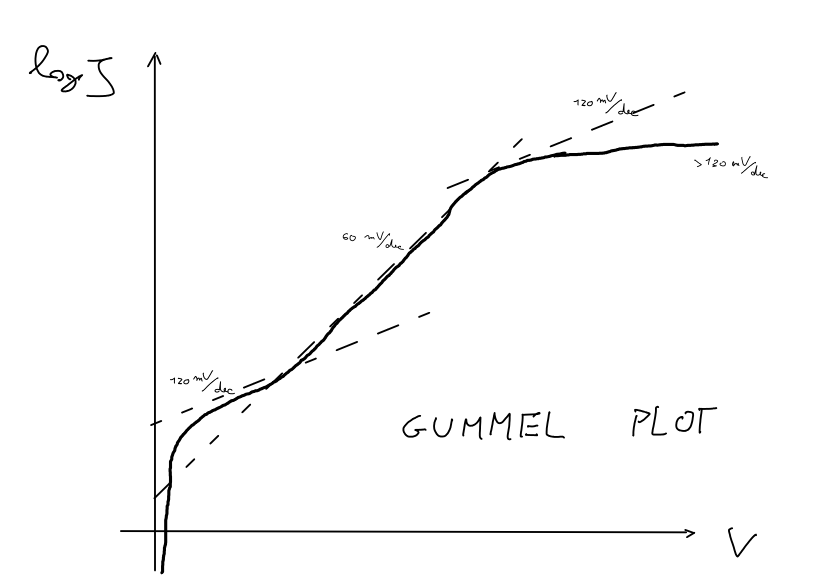
\includegraphics[width=0.5\textwidth]{gummel.png}\\
\raggedright

%------------------------------------------------------------------------%
\section{Small signal model}
%------------------------------------------------------------------------%
The pn junction is, of course, a non linear device if we assume that is polarized at $\overline{V}>0$ and we change that voltage of $\sigma V$ we are interested in its response. We have 3 small signal parameters: conductance, depletion capacitance and diffusion capacitance.
%------------------------------------------------------------------------%
\subsection{Conductance}
Changing the voltage of $\sigma V$ we have a variation of the current so a condctance that we can calculate as 
\begin{equation}
g_m=\frac{\partial I}{\partial V}=\frac{I}{kt/q}
\end{equation}
%------------------------------------------------------------------------%
\subsection{Deplition capacitance}
Changing $\delta V$ we remove a part of the depletion region as a consequence of majority injected in the junction that neutralize the fixed charges in the DL. We have a variation of the charge stored in the device as a consequence of a variation of the voltage so a capacitance.\\
We can introduce 
\begin{equation}
C_{dep}=\frac{\partial Q_{DL}}{\partial V}=-\frac{\partial }{\partial V}(qN_dx_n)=\frac{\varepsilon_{si}}{W_d}
\end{equation}
The minus sign is place in order to have a positive C and this formula is valid olso for non constant doping concentration.\\
%------------------------------------------------------------------------%
\subsection{Diffusion capacitance}
Olso in the quasi-neutral region we have charges stored that change if $\sigma V$ change due to the excess of minority. This capacitance is called diffusion capacitance and is defined as 
\begin{equation}
C_{diff}=\frac{\partial Q_{diff}}{\partial V}
\end{equation} 
we have therefore define $Q_{diff}$. Assuming forward bias and so neglecting $n_{p0}$ we can write $Q_{diff}=\int^{W_p}_0 q\Delta n(x) dx$.\\
For a wide base diode we have 
\begin{equation}
Q_{diff}=q\Delta n(0) \frac{L_n^2}{L_n}\frac{D_n}{D_n}=J_n\tau_n
\end{equation}
For a narrow base diode 
\begin{equation}
Q_{diff}=q\Delta n(0) \frac{W_p^2}{2W_p}\frac{D_n}{D_n}=J_nt_p
\end{equation}
where $t_p$ is defined as electron transit time through the quasi-neutral p region.\\

\begin{wrapfigure}{i}{0pt}
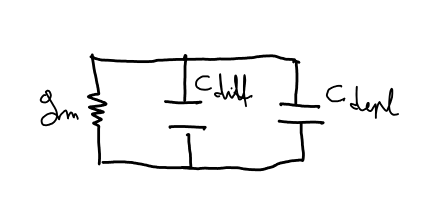
\includegraphics[width=0.35\textwidth]{smallpn.png}
\end{wrapfigure}

It's called like this beacuse from the current equation we can derive that $J_n=qD_n\Delta n(0)/W_p=q\Delta n(x) v_{diff}=q\Delta n(0)\frac{W_p-x}{W_p} v_{diff}$ from this we obtain $v_{diff}=\frac{D_n}{W_p-x}$ and from this integrating from 0 to $W_p$ in dx $\frac{1}{v_{diff}}$ we obtain exactly $t_p=\frac{W_p^2}{2D_n}$.\\
Going back to the diffusion capacitance we have for a wide base diode
\begin{equation}
C_{diff}^{wide}=g_m\tau_n
\end{equation} 
and for a narrow base
\begin{equation}
C_{diff}^{narrow}=g_mt_p
\end{equation}
In the end the small signal model is showed in figure.\\
In reverse bias the modulation of the quasi-neutral change is negligible and so is the diffusion capacitance.

